%-----------------------------------------------------------------------------%
\chapter{\babTiga}
%-----------------------------------------------------------------------------%
Bab ini akan menjelaskan rancangan sistem yang akan dibuat. Rancangan tersebut mencakup gambaran umum \plat~yang akan digunakan, gambaran umum \textit{gateway} beserta rancangan implementasinya, dan rancangan pengujian.

\section{Gambaran Umum Sistem}
Dalam tugas akhir ini, akan diimplementasikan sebuah \textit{gateway} yang akan menghubungkan jaringan lampu berbasis ZigBee dengan sebuah \plat~\iot~berbasis media sosial. Pada \plat~ini, seorang pengguna dapat menghubungkan berbagai perangkat  yang dimilikinya ke internet, dan kemudian memberikan informasi terkait perangkat tersebut ke teman-temannya di media sosial. Selain membagikan informasi terkait perangkat, pengguna juga dapat membagikan akses kontrol suatu perangkat ke internet atau teman-temannya di media sosial. Gambaran keseluruhan sistem ini dapat dilihat pada gambar \ref{fig:rancangan-siot}.

\begin{figure}
	\centering
	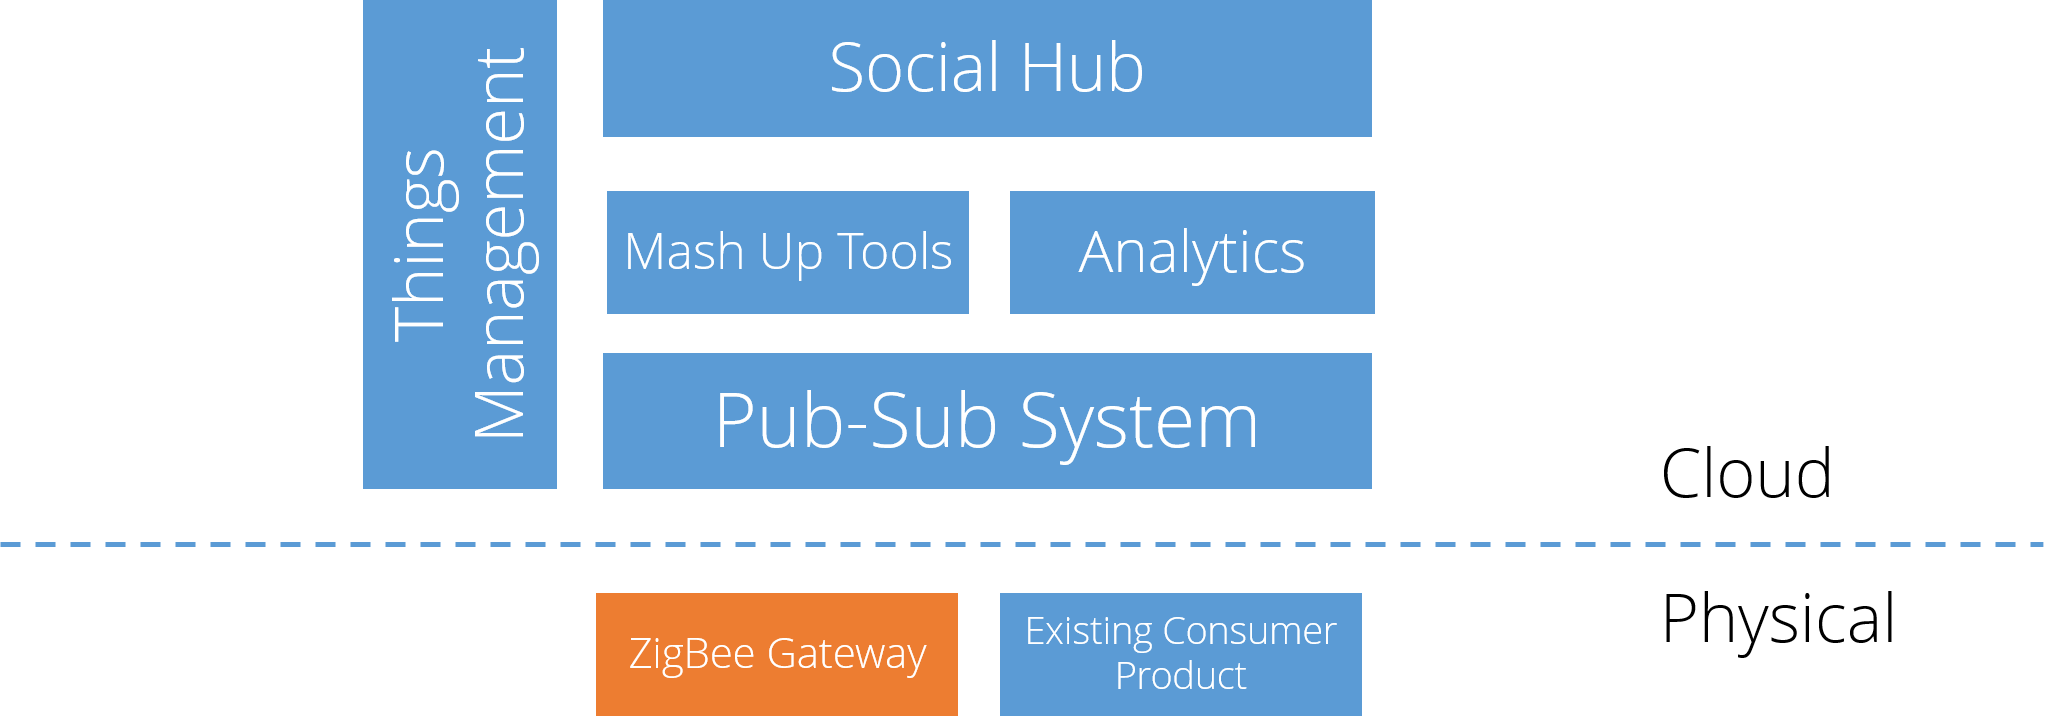
\includegraphics[width=.9\textwidth]{pics/rancangan-siot.PNG}
	\caption{Gambaran Umum \textit{Platform} \IOT~berbasis media sosial}
	\label{fig:rancangan-siot}
\end{figure}

Sistem ini terdiri dari beberapa bagian yang saling berhubungan. Sebagian besar sistem ini berada di server yang terhubung dengan jaringan internet. Penjelasan lebih detail mengenai bagian-bagian tersebut adalah sebagai berikut:
\begin{enumerate}
	\item \textit{Social Hub}
	
	Bagian ini merupakan abstraksi teratas dalam keseluruhan sistem. Bagian ini sekaligus menjadi \textit{user interface}, dimana penggunga \plat~nantinya akan mengakses sistem ini. Selain menjadi tempat pengguna mendaftar, bagian ini juga memiliki fungsi yang sangat penting, yaitu mengatur bagaimana mekanisme pembagian hak akses dan hak kontrol diantara seorang pengguna dengan pengguna lainnya. Sebagai contoh, pengguna dapat memilih apakah hak akses informasi mengenai sebuah perangkat yang dimilikinya akan dibagikan ke seluruh pengguna internet, hanya teman-temannya saja, atau hanya orang-orang tertentu saja.
	
	\item \textit{Widget}
	
	\textit{Widget} merupakan salah satu cara bagi pengguna \plat~untuk berinteraksi dengan suatu perangkat. Melalui \textit{widget}, pengguna dapat melakukan otomasi terhadap sebuah perangkat jika memenuhi kondisi tertentu. Misalnya, seorang pengguna dapat mengatur agar lampu ruang keluarga yang dimilikinya akan otomatis menyala jika pengguna mendapat email dengan subjek tertentu.
	
	\item \textit{Analytics}
	
	Dengan banyaknya perangkat yang nantinya akan terhubung ke \plat~ini, akan sangat banyak pula data yang melewati sistem ini. Data-data tersebut jika dilihat secara terpisah mungkin tidak memiliki nilai yang berarti. Namun, jika data seperti ini terdapat dalam jumlah yang sangat banyak, kita mungkin bisa mendapatkan wawasan tentang suatu hal yang terkait dengan data tersebut. Oleh karena itu, diperlukan suatu bagian yang dapat mengolah data yang banyak ini sehingga dapat memberikan suatu informasi yang berarti. Inilah peran dari bagian \textit{analytics}.
	
	\item \textit{Broker}
	
	Seperti yang telah disebutkan sebelumnya, seiring dengan semakin banyaknya pengguna yang terdaftar dan perangkat yang terhubung, akan semakin banyak pula data yang akan melewati sistem ini. Data-data ini harus dikirimkan dari satu perangkat ke setiap pengguna yang berhak menerimanya, dan juga dari pengguna ke setiap perangkat yang harus menerimanya. Oleh karena itu, diperlukan suatu mekanisme pengaturan pengiriman pesan, yang dapat mengirimkan setiap data tersebut ke tujuan yang sesuai dan tetap menjaga kualitas kinerja dari sistem. Hal terkait mekanisme pengiriman pesan inilah yang ditangani oleh \textit{broker}.
	
	\item \textit{Things Management}
	
	\textit{Things management} adalah bagian yang mengatur hubungan antara sistem ini dengan setiap perangkat yang terhubung. \textit{Things management} mengatur mulai dari proses pendaftaran perangkat, hingga penyimpanan informasi terkait perangkat. Things management ini juga yang mengatur bagaimana mekanisme komunikasi antara \plat~dengan perangkat. Perangkat yang terhubung dengan bagian ini terbagi menjadi dua macam. Yang pertama adalah perangkat yang sudah tersedia di pasaran saat ini. Untuk perangkat jenis ini, \textit{things management} akan menggunakan API perangkat terkait sebagai jalur komunikasi dengan perangkat tersebut. Dengan demikian, perangkat yang sudah dimiliki pengguna dapat langsung dihubungkan dengan \plat~ini. Jenis kedua adalah perangkat yang akan dikembangkan di masa depan. Untuk perangkat jenis ini, \textit{things management} akan menyediakan sebuah API yang dapat digunakan oleh pengembang perangkat cerdas, sehingga perangkat yang dikembangkannya dapat terhubung dengan \plat~ini.
	
	\item \textit{Gateway}
	
	Bagian yang terakhir adalah \textit{gateway}. Bagian ini berfungsi menghubungkan suatu perangkat dengan internet, khususnya \plat~ini. \textit{Gateway} inilah yang akan \saya~implementasikan dalam tugas akhir ini. Dalam sistem ini, \textit{gateway} akan berhubungan dengan \textit{things management} sebagai perangkat jenis kedua. Oleh karena itu, dalam melakukan implementasi \textit{gateway} ini \saya~akan mengacu pada API yang disediakan oleh \textit{things management}. Meskipun di masa mendatang diharapkan \textit{gateway} bisa menghubungkan berbagai jenis perangkat, namun untuk implementasi saat ini \saya~akan fokus pada perangkat lampu yang menggunakan teknologi ZigBee.
	
\end{enumerate}

\subsection{Gambaran Umum \textit{Gateway}}
\todo{
	Penjelasan mengenai gateway yang akan dibuat, termasuk perangkat yang digunakan. Jelaskan juga gambaran gateway yang udah dibuat sama farah.
	}
	
\section{Rancangan Implementasi \textit{Gateway}}
\todo{
	Penjelasan mendetail mengenai rancangan gateway
	\begin{itemize}
	\item spesifikiasi raspberry beserta isinya
	\item spesifikasi raspbee
	\item Tools yang digunakan
	\subitem deConz == jelaskan juga profile apa yang diimplementasikan oleh deConz
	\subitem apache server
	\subitem Mosquitto server
	\subitem eclipse paho
	\item Rancangan mekanisme pengiriman pesan
	\item Rancangan topik
	\item rancangan mekanisme penggunaan oleh user
	\subitem cara terhubung ke gateway
	\subitem cara menghubungkan device zigbee
	\subitem cara mengontrol device zigbee langsung dari gateway
	\subitem cara mendaftarkan device zigbee ke platform
	\item rancangan detil pesan, termasuk penjelasan semua fungsi zigbee light link
\end{itemize}
	}
	
\section{Rancangan Pengujian}

